% !TEX root = thesis_draft.tex

\section{General Discussion}

We investigated the sensitivity of a hyperscanning data analysis to different
methodological choices by performing an analysis of inter-brain synchrony (IBS)
data recorded during \textcite{newman_effects_2021}'s tacit coordination task.
We built a complete analysis pipeline that tested three IBS measures: the phase
locking value (PLV), the circular correlation coefficient (CCorr) and the
imaginary part of coherency (ImagCoh). Contrary to our expectations, we found
the analysis outcome to be sensitive to relatively minor changes to this
pipeline.

All studied measures of IBS rely on a frequency analysis
step to transform the raw EEG data into the frequency domain. We found that
varying the resolution of the output or the exact tapering method used to
control spectral leakage resulted in different IBS values. The CCorr
measure was especially sensitive to such changes. As long as you are comparing
apples to apples, i.e. only values that have been calculated with the same
methodology, this variation should not be a problem. But it is a reason to
caution against comparing raw IBS values across experiments or analyses. Using
statistical methods that can take this into account, like permutation tests
that will make the same assumptions when generating a null distribution, is
recommended.

\textcite{burgess_interpretation_2013} found the CCorr measure to be less
sensitive to detecting spurious IBS than other measures. Our study did not
encounter this issue, because the permutation tests did not detect any IBS. On
the other hand, our simulation study clearly illustrates
\textcite{kayhan_deep_2022}'s observation that PLV only measures the consistency
of the phase components of the EEG signals coming from each participant, not
whether they co-vary. Most strikingly, we see it completely ignore a strong
negative linear relation between the two phase components (see
Figure~\ref{fig:simulation_local_search}). The ImagCoh measure is hardest to
evaluate. It seems to be less sensitive in general to changes in
the data it is calculated upon. For example, in the simulation study, finding
examples for different ImagCoh values was harder than for the other measures.
Also, it only responded little to changes in the frequency analysis process. If
it still picks up on `real' effects, it would be the best measure tested. But
the fact that it is so insensitive, makes me doubtful about whether it would
quantify such effects. In the end, weighing all the evidence, I would prefer
using the CCorr measure for measuring IBS. But the PLV measure is also worth
considering considering. While it has its flaws, its ubiquitousness in the
hyperscanning literature makes it more familiar to the average reader.

\subsection{Contributions}

Next to the research project's results and pipeline description, we make
available validated implementations of the PLV, CCorr and ImagCoh measures for
both MATLAB and R. During the project, we also developed a MATLAB implementation
of \textcite{mahmood_robust_2022}'s robust circular correlation measure
(Algorithm~\ref{alg:robust}), although the implementation is slow and as
discussed previously the measure itself is not well-defined from a theoretical
point of view. Finally, in the end of the simulation study section, we
describe a way to perform a power analysis for tests used in IBS studies. It
reuses the method the simulation study uses to generate fake data for a given
IBS value (Algorithm \ref{alg:optimize-measures}). As a consequence, the
test will only have access to the phase component of the signal, as the
simulation study ignored amplitude components. But that can still be useful for
power analyses of tests that target phase-based measures only.

\subsection{Limitations}

This research project, especially the simulation study part, has been heavily
focused on phase-based IBS measures. The only exception is the ImagCoh measure.
\textcite{ayrolles_hypyp_2021} suggest phase-based measures are better at
measuring ``ongoing cognitive processing'', while amplitude-based measures are
better for measuring ``cognitive state''. It would be interesting to also
consider other amplitude-based measures, like the `power envelope correlation
between orthogonalized signals' measure described by
\textcite{hipp_large-scale_2012}. That measure is also used by
\textcite{dikker_crowdsourcing_2021}, who call it `projected power correlation'
instead. Another measure that was considered for inclusion in this study is the
Kraskov mutual information measure \parencite{kraskov_estimating_2004}.
\textcite{burgess_interpretation_2013} recommends it alongside the CCorr
measure. But while \citeauthor{burgess_interpretation_2013}'s work seems to have
single-handedly popularized the latter\footnote{Most discussions of the CCorr
measure I have seen can be traced back to
\textcite{burgess_interpretation_2013}'s work
\parencite[to name just a few]{chen_trait_2021,farahzadi_towards_2021,kurihara_relationship_2022,wikstrom_inter-brain_2022,goldstein_brain--brain_2018,kingsbury_multi-brain_2020}.},
the former seems to be have much less uptake. Perhaps it is due to the lack of
implementations being available
\footnote{\url{https://github.com/otoolej/mutual_info_kNN/blob/master/mi_cont_cont.m}
comes the closest, but it is does not match
\citeauthor{burgess_interpretation_2013}'s definition exactly. For one, it does
not use an angular distance metric.}, or the more complex
(information-theoretic) definitions. At least, that is the reason why it has not
been included in the present project.

Figures~\ref{fig:permutation_alpha},~\ref{fig:permutation_theta},~\ref{fig:slopes_alpha}~and~\ref{fig:slopes_theta}
use topographical plots of the scalp that are a common sight in EEG research.
While actual values are only available for the electrode sites, the visualization
fits a surface to them to present a continuous image. While interpreting some of
these figures during this project, this lead me to the wrong conclusions at
times. For example, it is common to see extreme values around the edges of the
scalp because the surface continues on outside the data's range for a bit. As a
result, I switched to drawing Voronoi cells around the electrodes instead when
analysing the prediction data (see
Figures~\ref{fig:logistic_coef}~and~\ref{fig:svm_indiv_topo}). Of course, this
approach also has its downsides. It will be less familiar to researchers in the
field, and the discrete nature of the visualization is unrealistic.

IBS permutation tests that generate their null hypothesis distribution by
shuffling dyads, as we did in the permutation test analysis section, are a nice
way to determine whether synchrony is just task-related, or due to cooperation
within the dyad. That said, if such a test yields a significant result, there
are other possible explanations. For example, if the two participants both have
a faster response time than other dyads, this could lead to the test finding
synchrony between them that is `just' due to their early motor response. Such a
response would be solely task-related, not due to the participants working
together or interacting otherwise. It is something to keep in mind when
designing IBS experiments.

\begin{figure}[!htpb]
  \resizebox{\linewidth}{!}{% Graphic for TeX using PGF
% Title: /home/marten/AI7/MasterProject/causal.dia
% Creator: Dia v0.97.3
% CreationDate: Thu Dec 15 02:02:04 2022
% For: marten
% \usepackage{tikz}
% The following commands are not supported in PSTricks at present
% We define them conditionally, so when they are implemented,
% this pgf file will use them.
\ifx\du\undefined
  \newlength{\du}
\fi
\setlength{\du}{15\unitlength}
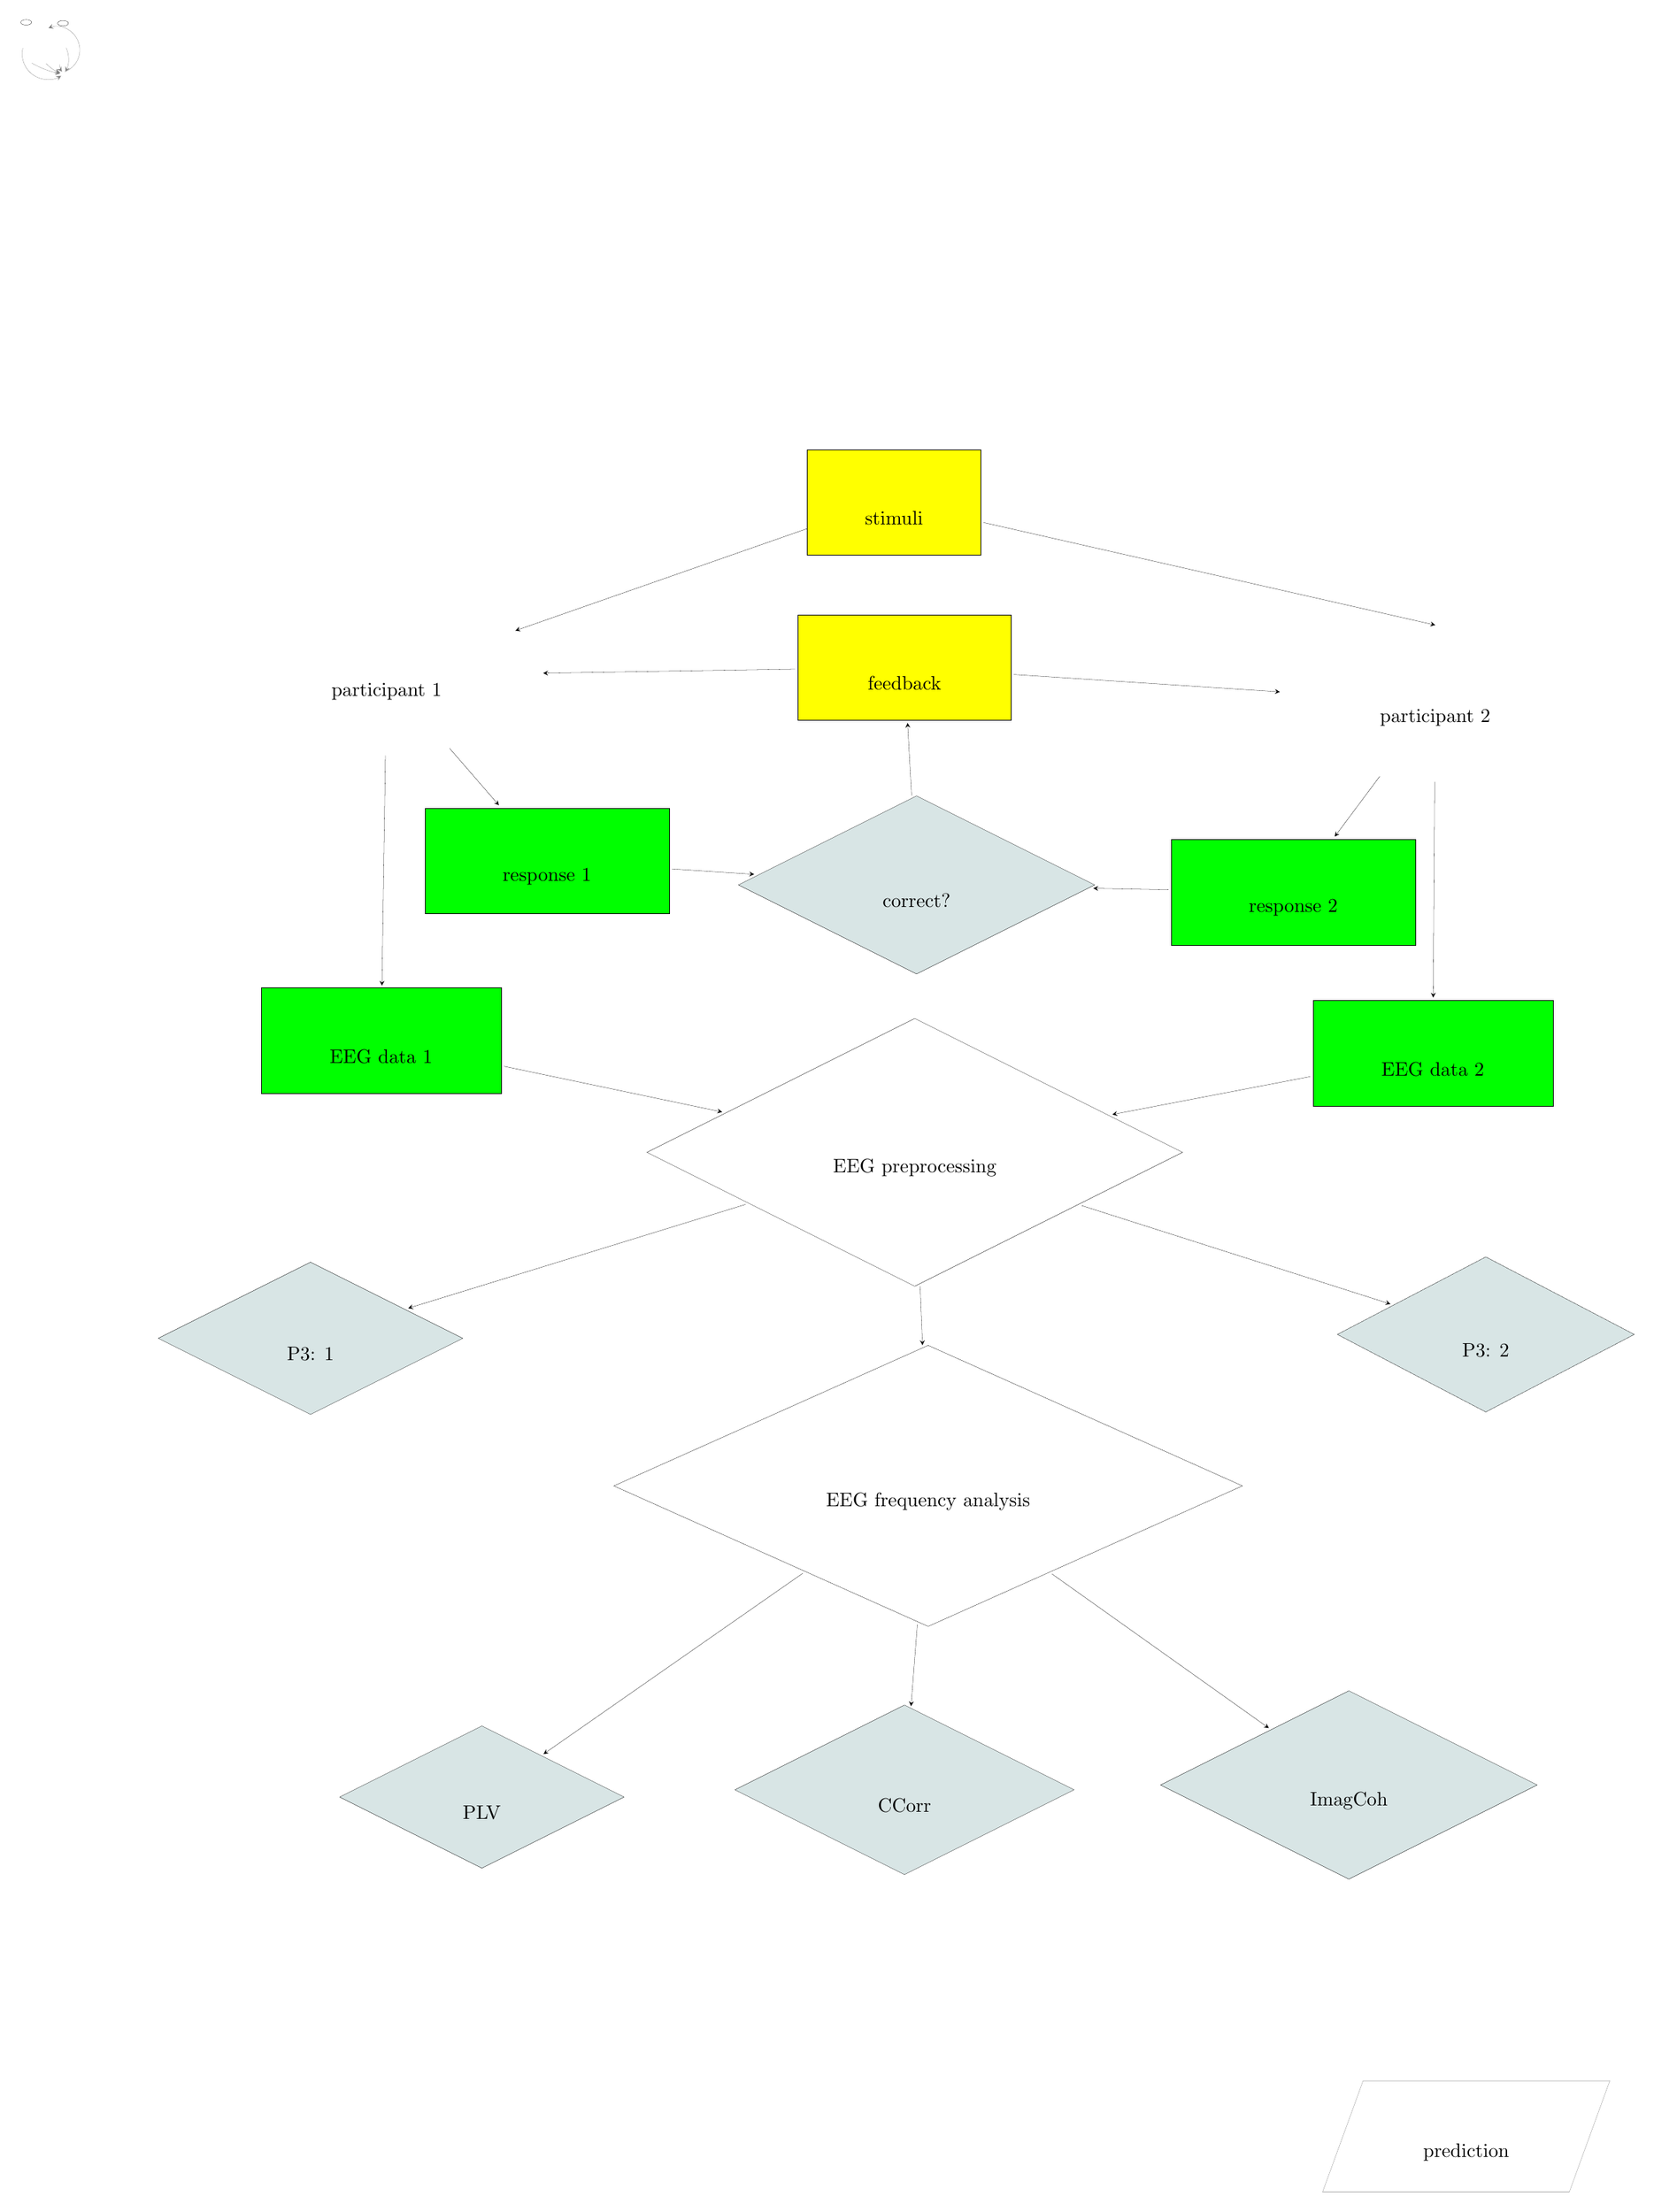
\begin{tikzpicture}
\pgftransformxscale{1.000000}
\pgftransformyscale{-1.000000}
\definecolor{dialinecolor}{rgb}{0.000000, 0.000000, 0.000000}
\pgfsetstrokecolor{dialinecolor}
\definecolor{dialinecolor}{rgb}{1.000000, 1.000000, 1.000000}
\pgfsetfillcolor{dialinecolor}
\definecolor{dialinecolor}{rgb}{1.000000, 1.000000, 1.000000}
\pgfsetfillcolor{dialinecolor}
\fill (24.287240\du,37.467200\du)--(28.725917\du,37.467200\du)--(27.997976\du,39.467200\du)--(23.559300\du,39.467200\du)--cycle;
\pgfsetlinewidth{0.100000\du}
\pgfsetdash{}{0pt}
\pgfsetdash{}{0pt}
\pgfsetmiterjoin
\definecolor{dialinecolor}{rgb}{0.498039, 0.498039, 0.498039}
\pgfsetstrokecolor{dialinecolor}
\draw (24.287240\du,37.467200\du)--(28.725917\du,37.467200\du)--(27.997976\du,39.467200\du)--(23.559300\du,39.467200\du)--cycle;
% setfont left to latex
\definecolor{dialinecolor}{rgb}{0.000000, 0.000000, 0.000000}
\pgfsetstrokecolor{dialinecolor}
\node at (26.142608\du,38.751360\du){prediction};
\pgfsetlinewidth{0.100000\du}
\pgfsetdash{}{0pt}
\pgfsetdash{}{0pt}
\pgfsetbuttcap
{
\definecolor{dialinecolor}{rgb}{0.498039, 0.498039, 0.498039}
\pgfsetfillcolor{dialinecolor}
% was here!!!
\pgfsetarrowsend{stealth}
\definecolor{dialinecolor}{rgb}{0.498039, 0.498039, 0.498039}
\pgfsetstrokecolor{dialinecolor}
\pgfpathmoveto{\pgfpoint{5.004066\du}{25.350989\du}}
\pgfpatharc{193}{59}{13.157261\du and 13.157261\du}
\pgfusepath{stroke}
}
\pgfsetlinewidth{0.100000\du}
\pgfsetdash{}{0pt}
\pgfsetdash{}{0pt}
\pgfsetbuttcap
{
\definecolor{dialinecolor}{rgb}{0.498039, 0.498039, 0.498039}
\pgfsetfillcolor{dialinecolor}
% was here!!!
\pgfsetarrowsend{stealth}
\definecolor{dialinecolor}{rgb}{0.498039, 0.498039, 0.498039}
\pgfsetstrokecolor{dialinecolor}
\pgfpathmoveto{\pgfpoint{9.657185\du}{33.076071\du}}
\pgfpatharc{120}{100}{44.359140\du and 44.359140\du}
\pgfusepath{stroke}
}
\pgfsetlinewidth{0.100000\du}
\pgfsetdash{}{0pt}
\pgfsetdash{}{0pt}
\pgfsetbuttcap
{
\definecolor{dialinecolor}{rgb}{0.498039, 0.498039, 0.498039}
\pgfsetfillcolor{dialinecolor}
% was here!!!
\pgfsetarrowsend{stealth}
\definecolor{dialinecolor}{rgb}{0.498039, 0.498039, 0.498039}
\pgfsetstrokecolor{dialinecolor}
\pgfpathmoveto{\pgfpoint{17.001187\du}{33.320496\du}}
\pgfpatharc{137}{110}{18.125522\du and 18.125522\du}
\pgfusepath{stroke}
}
\pgfsetlinewidth{0.100000\du}
\pgfsetdash{}{0pt}
\pgfsetdash{}{0pt}
\pgfsetbuttcap
{
\definecolor{dialinecolor}{rgb}{0.498039, 0.498039, 0.498039}
\pgfsetfillcolor{dialinecolor}
% was here!!!
\pgfsetarrowsend{stealth}
\definecolor{dialinecolor}{rgb}{0.498039, 0.498039, 0.498039}
\pgfsetstrokecolor{dialinecolor}
\pgfpathmoveto{\pgfpoint{23.827651\du}{33.786128\du}}
\pgfpatharc{180}{143}{6.054480\du and 6.054480\du}
\pgfusepath{stroke}
}
\pgfsetlinewidth{0.100000\du}
\pgfsetdash{}{0pt}
\pgfsetdash{}{0pt}
\pgfsetbuttcap
{
\definecolor{dialinecolor}{rgb}{0.498039, 0.498039, 0.498039}
\pgfsetfillcolor{dialinecolor}
% was here!!!
\pgfsetarrowsend{stealth}
\definecolor{dialinecolor}{rgb}{0.498039, 0.498039, 0.498039}
\pgfsetstrokecolor{dialinecolor}
\pgfpathmoveto{\pgfpoint{26.505631\du}{37.467573\du}}
\pgfpatharc{69}{-110}{11.947093\du and 11.947093\du}
\pgfusepath{stroke}
}
\definecolor{dialinecolor}{rgb}{1.000000, 1.000000, 0.000000}
\pgfsetfillcolor{dialinecolor}
\fill (14.286900\du,8.112710\du)--(14.286900\du,10.012710\du)--(17.411900\du,10.012710\du)--(17.411900\du,8.112710\du)--cycle;
\pgfsetlinewidth{0.100000\du}
\pgfsetdash{}{0pt}
\pgfsetdash{}{0pt}
\pgfsetmiterjoin
\definecolor{dialinecolor}{rgb}{0.000000, 0.000000, 0.000000}
\pgfsetstrokecolor{dialinecolor}
\draw (14.286900\du,8.112710\du)--(14.286900\du,10.012710\du)--(17.411900\du,10.012710\du)--(17.411900\du,8.112710\du)--cycle;
% setfont left to latex
\definecolor{dialinecolor}{rgb}{0.000000, 0.000000, 0.000000}
\pgfsetstrokecolor{dialinecolor}
\node at (15.849400\du,9.346870\du){stimuli};
\definecolor{dialinecolor}{rgb}{1.000000, 1.000000, 0.000000}
\pgfsetfillcolor{dialinecolor}
\fill (14.119700\du,11.084400\du)--(14.119700\du,12.984400\du)--(17.954700\du,12.984400\du)--(17.954700\du,11.084400\du)--cycle;
\pgfsetlinewidth{0.100000\du}
\pgfsetdash{}{0pt}
\pgfsetdash{}{0pt}
\pgfsetmiterjoin
\definecolor{dialinecolor}{rgb}{0.000000, 0.000000, 0.000000}
\pgfsetstrokecolor{dialinecolor}
\draw (14.119700\du,11.084400\du)--(14.119700\du,12.984400\du)--(17.954700\du,12.984400\du)--(17.954700\du,11.084400\du)--cycle;
% setfont left to latex
\definecolor{dialinecolor}{rgb}{0.000000, 0.000000, 0.000000}
\pgfsetstrokecolor{dialinecolor}
\node at (16.037200\du,12.318560\du){feedback};
\definecolor{dialinecolor}{rgb}{1.000000, 1.000000, 1.000000}
\pgfsetfillcolor{dialinecolor}
\pgfpathellipse{\pgfpoint{6.720752\du}{12.183961\du}}{\pgfpoint{2.769322\du}{0\du}}{\pgfpoint{0\du}{1.384661\du}}
\pgfusepath{fill}
\pgfsetlinewidth{0.100000\du}
\pgfsetdash{}{0pt}
\pgfsetdash{}{0pt}
\pgfsetmiterjoin
\definecolor{dialinecolor}{rgb}{0.000000, 0.000000, 0.000000}
\pgfsetstrokecolor{dialinecolor}
\pgfpathellipse{\pgfpoint{6.720752\du}{12.183961\du}}{\pgfpoint{2.769322\du}{0\du}}{\pgfpoint{0\du}{1.384661\du}}
\pgfusepath{stroke}
% setfont left to latex
\definecolor{dialinecolor}{rgb}{0.000000, 0.000000, 0.000000}
\pgfsetstrokecolor{dialinecolor}
\node at (6.720752\du,12.468121\du){participant 1};
\definecolor{dialinecolor}{rgb}{1.000000, 1.000000, 1.000000}
\pgfsetfillcolor{dialinecolor}
\pgfpathellipse{\pgfpoint{25.584822\du}{12.657761\du}}{\pgfpoint{2.769322\du}{0\du}}{\pgfpoint{0\du}{1.384661\du}}
\pgfusepath{fill}
\pgfsetlinewidth{0.100000\du}
\pgfsetdash{}{0pt}
\pgfsetdash{}{0pt}
\pgfsetmiterjoin
\definecolor{dialinecolor}{rgb}{0.000000, 0.000000, 0.000000}
\pgfsetstrokecolor{dialinecolor}
\pgfpathellipse{\pgfpoint{25.584822\du}{12.657761\du}}{\pgfpoint{2.769322\du}{0\du}}{\pgfpoint{0\du}{1.384661\du}}
\pgfusepath{stroke}
% setfont left to latex
\definecolor{dialinecolor}{rgb}{0.000000, 0.000000, 0.000000}
\pgfsetstrokecolor{dialinecolor}
\node at (25.584822\du,12.941921\du){participant 2};
\pgfsetlinewidth{0.100000\du}
\pgfsetdash{}{0pt}
\pgfsetdash{}{0pt}
\pgfsetbuttcap
{
\definecolor{dialinecolor}{rgb}{0.000000, 0.000000, 0.000000}
\pgfsetfillcolor{dialinecolor}
% was here!!!
\pgfsetarrowsend{stealth}
\definecolor{dialinecolor}{rgb}{0.000000, 0.000000, 0.000000}
\pgfsetstrokecolor{dialinecolor}
\draw (14.286900\du,9.537710\du)--(9.037608\du,11.373644\du);
}
\pgfsetlinewidth{0.100000\du}
\pgfsetdash{}{0pt}
\pgfsetdash{}{0pt}
\pgfsetbuttcap
{
\definecolor{dialinecolor}{rgb}{0.000000, 0.000000, 0.000000}
\pgfsetfillcolor{dialinecolor}
% was here!!!
\pgfsetarrowsend{stealth}
\definecolor{dialinecolor}{rgb}{0.000000, 0.000000, 0.000000}
\pgfsetstrokecolor{dialinecolor}
\draw (17.461469\du,9.428725\du)--(25.584800\du,11.273100\du);
}
\pgfsetlinewidth{0.100000\du}
\pgfsetdash{}{0pt}
\pgfsetdash{}{0pt}
\pgfsetbuttcap
{
\definecolor{dialinecolor}{rgb}{0.000000, 0.000000, 0.000000}
\pgfsetfillcolor{dialinecolor}
% was here!!!
\pgfsetarrowsend{stealth}
\definecolor{dialinecolor}{rgb}{0.000000, 0.000000, 0.000000}
\pgfsetstrokecolor{dialinecolor}
\draw (14.069453\du,12.065989\du)--(9.537749\du,12.138739\du);
}
\pgfsetlinewidth{0.100000\du}
\pgfsetdash{}{0pt}
\pgfsetdash{}{0pt}
\pgfsetbuttcap
{
\definecolor{dialinecolor}{rgb}{0.000000, 0.000000, 0.000000}
\pgfsetfillcolor{dialinecolor}
% was here!!!
\pgfsetarrowsend{stealth}
\definecolor{dialinecolor}{rgb}{0.000000, 0.000000, 0.000000}
\pgfsetstrokecolor{dialinecolor}
\draw (18.005115\du,12.162885\du)--(22.789415\du,12.475250\du);
}
\definecolor{dialinecolor}{rgb}{0.000000, 1.000000, 0.000000}
\pgfsetfillcolor{dialinecolor}
\fill (7.409660\du,14.564600\du)--(7.409660\du,16.464600\du)--(11.804660\du,16.464600\du)--(11.804660\du,14.564600\du)--cycle;
\pgfsetlinewidth{0.100000\du}
\pgfsetdash{}{0pt}
\pgfsetdash{}{0pt}
\pgfsetmiterjoin
\definecolor{dialinecolor}{rgb}{0.000000, 0.000000, 0.000000}
\pgfsetstrokecolor{dialinecolor}
\draw (7.409660\du,14.564600\du)--(7.409660\du,16.464600\du)--(11.804660\du,16.464600\du)--(11.804660\du,14.564600\du)--cycle;
% setfont left to latex
\definecolor{dialinecolor}{rgb}{0.000000, 0.000000, 0.000000}
\pgfsetstrokecolor{dialinecolor}
\node at (9.607160\du,15.798760\du){response 1};
\definecolor{dialinecolor}{rgb}{0.000000, 1.000000, 0.000000}
\pgfsetfillcolor{dialinecolor}
\fill (20.835000\du,15.129400\du)--(20.835000\du,17.029400\du)--(25.230000\du,17.029400\du)--(25.230000\du,15.129400\du)--cycle;
\pgfsetlinewidth{0.100000\du}
\pgfsetdash{}{0pt}
\pgfsetdash{}{0pt}
\pgfsetmiterjoin
\definecolor{dialinecolor}{rgb}{0.000000, 0.000000, 0.000000}
\pgfsetstrokecolor{dialinecolor}
\draw (20.835000\du,15.129400\du)--(20.835000\du,17.029400\du)--(25.230000\du,17.029400\du)--(25.230000\du,15.129400\du)--cycle;
% setfont left to latex
\definecolor{dialinecolor}{rgb}{0.000000, 0.000000, 0.000000}
\pgfsetstrokecolor{dialinecolor}
\node at (23.032500\du,16.363560\du){response 2};
\pgfsetlinewidth{0.100000\du}
\pgfsetdash{}{0pt}
\pgfsetdash{}{0pt}
\pgfsetbuttcap
{
\definecolor{dialinecolor}{rgb}{0.000000, 0.000000, 0.000000}
\pgfsetfillcolor{dialinecolor}
% was here!!!
\pgfsetarrowsend{stealth}
\definecolor{dialinecolor}{rgb}{0.000000, 0.000000, 0.000000}
\pgfsetstrokecolor{dialinecolor}
\draw (7.854245\du,13.491904\du)--(8.741097\du,14.515246\du);
}
\pgfsetlinewidth{0.100000\du}
\pgfsetdash{}{0pt}
\pgfsetdash{}{0pt}
\pgfsetbuttcap
{
\definecolor{dialinecolor}{rgb}{0.000000, 0.000000, 0.000000}
\pgfsetfillcolor{dialinecolor}
% was here!!!
\pgfsetarrowsend{stealth}
\definecolor{dialinecolor}{rgb}{0.000000, 0.000000, 0.000000}
\pgfsetstrokecolor{dialinecolor}
\draw (24.587042\du,13.995383\du)--(23.778381\du,15.079473\du);
}
\definecolor{dialinecolor}{rgb}{0.847059, 0.898039, 0.898039}
\pgfsetfillcolor{dialinecolor}
\fill (16.254610\du,14.346800\du)--(19.459020\du,15.949005\du)--(16.254610\du,17.551210\du)--(13.050200\du,15.949005\du)--cycle;
\pgfsetlinewidth{0.100000\du}
\pgfsetdash{}{0pt}
\pgfsetdash{}{0pt}
\pgfsetmiterjoin
\definecolor{dialinecolor}{rgb}{0.000000, 0.000000, 0.000000}
\pgfsetstrokecolor{dialinecolor}
\draw (16.254610\du,14.346800\du)--(19.459020\du,15.949005\du)--(16.254610\du,17.551210\du)--(13.050200\du,15.949005\du)--cycle;
% setfont left to latex
\definecolor{dialinecolor}{rgb}{0.000000, 0.000000, 0.000000}
\pgfsetstrokecolor{dialinecolor}
\node at (16.254610\du,16.233165\du){correct?};
\pgfsetlinewidth{0.100000\du}
\pgfsetdash{}{0pt}
\pgfsetdash{}{0pt}
\pgfsetbuttcap
{
\definecolor{dialinecolor}{rgb}{0.000000, 0.000000, 0.000000}
\pgfsetfillcolor{dialinecolor}
% was here!!!
\pgfsetarrowsend{stealth}
\definecolor{dialinecolor}{rgb}{0.000000, 0.000000, 0.000000}
\pgfsetstrokecolor{dialinecolor}
\draw (11.854083\du,15.661434\du)--(13.332556\du,15.758051\du);
}
\pgfsetlinewidth{0.100000\du}
\pgfsetdash{}{0pt}
\pgfsetdash{}{0pt}
\pgfsetbuttcap
{
\definecolor{dialinecolor}{rgb}{0.000000, 0.000000, 0.000000}
\pgfsetfillcolor{dialinecolor}
% was here!!!
\pgfsetarrowsend{stealth}
\definecolor{dialinecolor}{rgb}{0.000000, 0.000000, 0.000000}
\pgfsetstrokecolor{dialinecolor}
\draw (20.784925\du,16.036161\du)--(19.435056\du,16.010191\du);
}
\pgfsetlinewidth{0.100000\du}
\pgfsetdash{}{0pt}
\pgfsetdash{}{0pt}
\pgfsetbuttcap
{
\definecolor{dialinecolor}{rgb}{0.000000, 0.000000, 0.000000}
\pgfsetfillcolor{dialinecolor}
% was here!!!
\pgfsetarrowsend{stealth}
\definecolor{dialinecolor}{rgb}{0.000000, 0.000000, 0.000000}
\pgfsetstrokecolor{dialinecolor}
\draw (16.165305\du,14.341016\du)--(16.092747\du,13.034555\du);
}
\pgfsetlinewidth{0.100000\du}
\pgfsetdash{}{0pt}
\pgfsetdash{}{0pt}
\pgfsetbuttcap
{
\definecolor{dialinecolor}{rgb}{0.000000, 0.000000, 0.000000}
\pgfsetfillcolor{dialinecolor}
% was here!!!
\pgfsetarrowsend{stealth}
\definecolor{dialinecolor}{rgb}{0.000000, 0.000000, 0.000000}
\pgfsetstrokecolor{dialinecolor}
\draw (6.699028\du,13.618905\du)--(6.636308\du,17.761850\du);
}
\pgfsetlinewidth{0.100000\du}
\pgfsetdash{}{0pt}
\pgfsetdash{}{0pt}
\pgfsetbuttcap
{
\definecolor{dialinecolor}{rgb}{0.000000, 0.000000, 0.000000}
\pgfsetfillcolor{dialinecolor}
% was here!!!
\pgfsetarrowsend{stealth}
\definecolor{dialinecolor}{rgb}{0.000000, 0.000000, 0.000000}
\pgfsetstrokecolor{dialinecolor}
\draw (25.575267\du,14.092571\du)--(25.549409\du,17.975544\du);
}
\definecolor{dialinecolor}{rgb}{0.000000, 1.000000, 0.000000}
\pgfsetfillcolor{dialinecolor}
\fill (4.462610\du,17.799200\du)--(4.462610\du,19.699200\du)--(8.780110\du,19.699200\du)--(8.780110\du,17.799200\du)--cycle;
\pgfsetlinewidth{0.100000\du}
\pgfsetdash{}{0pt}
\pgfsetdash{}{0pt}
\pgfsetmiterjoin
\definecolor{dialinecolor}{rgb}{0.000000, 0.000000, 0.000000}
\pgfsetstrokecolor{dialinecolor}
\draw (4.462610\du,17.799200\du)--(4.462610\du,19.699200\du)--(8.780110\du,19.699200\du)--(8.780110\du,17.799200\du)--cycle;
% setfont left to latex
\definecolor{dialinecolor}{rgb}{0.000000, 0.000000, 0.000000}
\pgfsetstrokecolor{dialinecolor}
\node at (6.621360\du,19.033360\du){EEG data 1};
\definecolor{dialinecolor}{rgb}{0.000000, 1.000000, 0.000000}
\pgfsetfillcolor{dialinecolor}
\fill (23.384000\du,18.025400\du)--(23.384000\du,19.925400\du)--(27.701500\du,19.925400\du)--(27.701500\du,18.025400\du)--cycle;
\pgfsetlinewidth{0.100000\du}
\pgfsetdash{}{0pt}
\pgfsetdash{}{0pt}
\pgfsetmiterjoin
\definecolor{dialinecolor}{rgb}{0.000000, 0.000000, 0.000000}
\pgfsetstrokecolor{dialinecolor}
\draw (23.384000\du,18.025400\du)--(23.384000\du,19.925400\du)--(27.701500\du,19.925400\du)--(27.701500\du,18.025400\du)--cycle;
% setfont left to latex
\definecolor{dialinecolor}{rgb}{0.000000, 0.000000, 0.000000}
\pgfsetstrokecolor{dialinecolor}
\node at (25.542750\du,19.259560\du){EEG data 2};
\definecolor{dialinecolor}{rgb}{1.000000, 1.000000, 1.000000}
\pgfsetfillcolor{dialinecolor}
\fill (16.462669\du,24.234300\du)--(22.117037\du,26.762637\du)--(16.462669\du,29.290975\du)--(10.808300\du,26.762637\du)--cycle;
\pgfsetlinewidth{0.100000\du}
\pgfsetdash{}{0pt}
\pgfsetdash{}{0pt}
\pgfsetmiterjoin
\definecolor{dialinecolor}{rgb}{0.000000, 0.000000, 0.000000}
\pgfsetstrokecolor{dialinecolor}
\draw (16.462669\du,24.234300\du)--(22.117037\du,26.762637\du)--(16.462669\du,29.290975\du)--(10.808300\du,26.762637\du)--cycle;
% setfont left to latex
\definecolor{dialinecolor}{rgb}{0.000000, 0.000000, 0.000000}
\pgfsetstrokecolor{dialinecolor}
\node at (16.462669\du,27.046798\du){EEG frequency analysis};
\definecolor{dialinecolor}{rgb}{0.847059, 0.898039, 0.898039}
\pgfsetfillcolor{dialinecolor}
\fill (8.434070\du,31.082300\du)--(10.992230\du,32.361380\du)--(8.434070\du,33.640460\du)--(5.875910\du,32.361380\du)--cycle;
\pgfsetlinewidth{0.100000\du}
\pgfsetdash{}{0pt}
\pgfsetdash{}{0pt}
\pgfsetmiterjoin
\definecolor{dialinecolor}{rgb}{0.000000, 0.000000, 0.000000}
\pgfsetstrokecolor{dialinecolor}
\draw (8.434070\du,31.082300\du)--(10.992230\du,32.361380\du)--(8.434070\du,33.640460\du)--(5.875910\du,32.361380\du)--cycle;
% setfont left to latex
\definecolor{dialinecolor}{rgb}{0.000000, 0.000000, 0.000000}
\pgfsetstrokecolor{dialinecolor}
\node at (8.434070\du,32.645540\du){PLV};
\pgfsetlinewidth{0.100000\du}
\pgfsetdash{}{0pt}
\pgfsetdash{}{0pt}
\pgfsetbuttcap
{
\definecolor{dialinecolor}{rgb}{0.000000, 0.000000, 0.000000}
\pgfsetfillcolor{dialinecolor}
% was here!!!
\pgfsetarrowsend{stealth}
\definecolor{dialinecolor}{rgb}{0.000000, 0.000000, 0.000000}
\pgfsetstrokecolor{dialinecolor}
\draw (14.210016\du,28.333525\du)--(9.543981\du,31.587384\du);
}
\definecolor{dialinecolor}{rgb}{0.847059, 0.898039, 0.898039}
\pgfsetfillcolor{dialinecolor}
\fill (16.037460\du,30.705700\du)--(19.088120\du,32.231030\du)--(16.037460\du,33.756360\du)--(12.986800\du,32.231030\du)--cycle;
\pgfsetlinewidth{0.100000\du}
\pgfsetdash{}{0pt}
\pgfsetdash{}{0pt}
\pgfsetmiterjoin
\definecolor{dialinecolor}{rgb}{0.000000, 0.000000, 0.000000}
\pgfsetstrokecolor{dialinecolor}
\draw (16.037460\du,30.705700\du)--(19.088120\du,32.231030\du)--(16.037460\du,33.756360\du)--(12.986800\du,32.231030\du)--cycle;
% setfont left to latex
\definecolor{dialinecolor}{rgb}{0.000000, 0.000000, 0.000000}
\pgfsetstrokecolor{dialinecolor}
\node at (16.037460\du,32.515190\du){CCorr};
\pgfsetlinewidth{0.100000\du}
\pgfsetdash{}{0pt}
\pgfsetdash{}{0pt}
\pgfsetbuttcap
{
\definecolor{dialinecolor}{rgb}{0.000000, 0.000000, 0.000000}
\pgfsetfillcolor{dialinecolor}
% was here!!!
\pgfsetarrowsend{stealth}
\definecolor{dialinecolor}{rgb}{0.000000, 0.000000, 0.000000}
\pgfsetstrokecolor{dialinecolor}
\draw (16.268906\du,29.254521\du)--(16.154559\du,30.725086\du);
}
\definecolor{dialinecolor}{rgb}{0.847059, 0.898039, 0.898039}
\pgfsetfillcolor{dialinecolor}
\fill (24.031760\du,30.450100\du)--(27.419920\du,32.144180\du)--(24.031760\du,33.838260\du)--(20.643600\du,32.144180\du)--cycle;
\pgfsetlinewidth{0.100000\du}
\pgfsetdash{}{0pt}
\pgfsetdash{}{0pt}
\pgfsetmiterjoin
\definecolor{dialinecolor}{rgb}{0.000000, 0.000000, 0.000000}
\pgfsetstrokecolor{dialinecolor}
\draw (24.031760\du,30.450100\du)--(27.419920\du,32.144180\du)--(24.031760\du,33.838260\du)--(20.643600\du,32.144180\du)--cycle;
% setfont left to latex
\definecolor{dialinecolor}{rgb}{0.000000, 0.000000, 0.000000}
\pgfsetstrokecolor{dialinecolor}
\node at (24.031760\du,32.428340\du){ImagCoh};
\pgfsetlinewidth{0.100000\du}
\pgfsetdash{}{0pt}
\pgfsetdash{}{0pt}
\pgfsetbuttcap
{
\definecolor{dialinecolor}{rgb}{0.000000, 0.000000, 0.000000}
\pgfsetfillcolor{dialinecolor}
% was here!!!
\pgfsetarrowsend{stealth}
\definecolor{dialinecolor}{rgb}{0.000000, 0.000000, 0.000000}
\pgfsetstrokecolor{dialinecolor}
\draw (18.688491\du,28.345174\du)--(22.591766\du,31.120360\du);
}
\definecolor{dialinecolor}{rgb}{1.000000, 1.000000, 1.000000}
\pgfsetfillcolor{dialinecolor}
\fill (16.222060\du,18.351800\du)--(21.040220\du,20.760880\du)--(16.222060\du,23.169960\du)--(11.403900\du,20.760880\du)--cycle;
\pgfsetlinewidth{0.100000\du}
\pgfsetdash{}{0pt}
\pgfsetdash{}{0pt}
\pgfsetmiterjoin
\definecolor{dialinecolor}{rgb}{0.000000, 0.000000, 0.000000}
\pgfsetstrokecolor{dialinecolor}
\draw (16.222060\du,18.351800\du)--(21.040220\du,20.760880\du)--(16.222060\du,23.169960\du)--(11.403900\du,20.760880\du)--cycle;
% setfont left to latex
\definecolor{dialinecolor}{rgb}{0.000000, 0.000000, 0.000000}
\pgfsetstrokecolor{dialinecolor}
\node at (16.222060\du,21.045040\du){EEG preprocessing};
\pgfsetlinewidth{0.100000\du}
\pgfsetdash{}{0pt}
\pgfsetdash{}{0pt}
\pgfsetbuttcap
{
\definecolor{dialinecolor}{rgb}{0.000000, 0.000000, 0.000000}
\pgfsetfillcolor{dialinecolor}
% was here!!!
\pgfsetarrowsend{stealth}
\definecolor{dialinecolor}{rgb}{0.000000, 0.000000, 0.000000}
\pgfsetstrokecolor{dialinecolor}
\draw (8.829920\du,19.211970\du)--(12.756573\du,20.034740\du);
}
\pgfsetlinewidth{0.100000\du}
\pgfsetdash{}{0pt}
\pgfsetdash{}{0pt}
\pgfsetbuttcap
{
\definecolor{dialinecolor}{rgb}{0.000000, 0.000000, 0.000000}
\pgfsetfillcolor{dialinecolor}
% was here!!!
\pgfsetarrowsend{stealth}
\definecolor{dialinecolor}{rgb}{0.000000, 0.000000, 0.000000}
\pgfsetstrokecolor{dialinecolor}
\draw (23.334320\du,19.398449\du)--(19.777621\du,20.079773\du);
}
\pgfsetlinewidth{0.100000\du}
\pgfsetdash{}{0pt}
\pgfsetdash{}{0pt}
\pgfsetbuttcap
{
\definecolor{dialinecolor}{rgb}{0.000000, 0.000000, 0.000000}
\pgfsetfillcolor{dialinecolor}
% was here!!!
\pgfsetarrowsend{stealth}
\definecolor{dialinecolor}{rgb}{0.000000, 0.000000, 0.000000}
\pgfsetstrokecolor{dialinecolor}
\draw (16.318706\du,23.171620\du)--(16.361132\du,24.229913\du);
}
\definecolor{dialinecolor}{rgb}{0.847059, 0.898039, 0.898039}
\pgfsetfillcolor{dialinecolor}
\fill (5.351573\du,22.737300\du)--(8.090983\du,24.107005\du)--(5.351573\du,25.476710\du)--(2.612163\du,24.107005\du)--cycle;
\pgfsetlinewidth{0.100000\du}
\pgfsetdash{}{0pt}
\pgfsetdash{}{0pt}
\pgfsetmiterjoin
\definecolor{dialinecolor}{rgb}{0.000000, 0.000000, 0.000000}
\pgfsetstrokecolor{dialinecolor}
\draw (5.351573\du,22.737300\du)--(8.090983\du,24.107005\du)--(5.351573\du,25.476710\du)--(2.612163\du,24.107005\du)--cycle;
% setfont left to latex
\definecolor{dialinecolor}{rgb}{0.000000, 0.000000, 0.000000}
\pgfsetstrokecolor{dialinecolor}
\node at (5.351573\du,24.391165\du){P3: 1};
\definecolor{dialinecolor}{rgb}{0.847059, 0.898039, 0.898039}
\pgfsetfillcolor{dialinecolor}
\fill (26.495222\du,22.642400\du)--(29.165543\du,24.037537\du)--(26.495222\du,25.432674\du)--(23.824900\du,24.037537\du)--cycle;
\pgfsetlinewidth{0.100000\du}
\pgfsetdash{}{0pt}
\pgfsetdash{}{0pt}
\pgfsetmiterjoin
\definecolor{dialinecolor}{rgb}{0.000000, 0.000000, 0.000000}
\pgfsetstrokecolor{dialinecolor}
\draw (26.495222\du,22.642400\du)--(29.165543\du,24.037537\du)--(26.495222\du,25.432674\du)--(23.824900\du,24.037537\du)--cycle;
% setfont left to latex
\definecolor{dialinecolor}{rgb}{0.000000, 0.000000, 0.000000}
\pgfsetstrokecolor{dialinecolor}
\node at (26.495222\du,24.321697\du){P3: 2};
\pgfsetlinewidth{0.100000\du}
\pgfsetdash{}{0pt}
\pgfsetdash{}{0pt}
\pgfsetbuttcap
{
\definecolor{dialinecolor}{rgb}{0.000000, 0.000000, 0.000000}
\pgfsetfillcolor{dialinecolor}
% was here!!!
\pgfsetarrowsend{stealth}
\definecolor{dialinecolor}{rgb}{0.000000, 0.000000, 0.000000}
\pgfsetstrokecolor{dialinecolor}
\draw (13.177674\du,21.697995\du)--(7.109137\du,23.565996\du);
}
\pgfsetlinewidth{0.100000\du}
\pgfsetdash{}{0pt}
\pgfsetdash{}{0pt}
\pgfsetbuttcap
{
\definecolor{dialinecolor}{rgb}{0.000000, 0.000000, 0.000000}
\pgfsetfillcolor{dialinecolor}
% was here!!!
\pgfsetarrowsend{stealth}
\definecolor{dialinecolor}{rgb}{0.000000, 0.000000, 0.000000}
\pgfsetstrokecolor{dialinecolor}
\draw (19.224878\du,21.718638\du)--(24.778430\du,23.489961\du);
}
\pgfsetlinewidth{0.100000\du}
\pgfsetdash{}{0pt}
\pgfsetdash{}{0pt}
\pgfsetbuttcap
{
\definecolor{dialinecolor}{rgb}{0.498039, 0.498039, 0.498039}
\pgfsetfillcolor{dialinecolor}
% was here!!!
\pgfsetarrowsstart{stealth}
\definecolor{dialinecolor}{rgb}{0.498039, 0.498039, 0.498039}
\pgfsetstrokecolor{dialinecolor}
\pgfpathmoveto{\pgfpoint{26.749101\du}{37.418338\du}}
\pgfpatharc{28}{-24}{13.961809\du and 13.961809\du}
\pgfusepath{stroke}
}
\end{tikzpicture}
}
  \caption{A diagram of the causal structure of \textcite{newman_effects_2021}'s experimental setup, and its interaction with the accuracy classifiers described in this thesis. Stimuli are shown in yellow, while recorded measurements are shown in green. Calculated values are shown in grey.}
  \label{fig:causal}
\end{figure}

Finally, it is worth reflecting a bit on the prediction task. Considering that
we did not find significant IBS previously, it always was a long shot. But even
if we had, it is worth mapping out the causal path that would lead to a correct
prediction in \textcite{newman_effects_2021}'s task. See Appendix~\ref{app:task}
for more information about the task. Figure~\ref{fig:causal} does exactly that.
When a stimulus comes in, both participants give a response, and get feedback
based on if they both picked the same image or shape. They use that feedback to
adjust their mental model of what the other is doing, which they will use in
future trials. We record their brain activity while that is going on, run it
through the IBS pipeline, and get out IBS values (PLV, CCorr \& ImagCoh in the
diagram) and normal EEG values (P3 single trial ERP values). These are then in
turn used by the classifier to make a prediction of the accuracy in the current
trial. Now, what would be the mechanism that increases the odds of predicting
whether the dyad chose the same image or shape?

There are multiple possible ways. Theoretically, a group of images or shapes dissimilar to
previous examples could lead to a P3 ERP, and would most likely decrease their
chances of picking the same image or shape. But as the images are similar switching only
their colours, such an advantage would be unlikely to last long. Alternatively,
one of the participants could `simulate' what the other is doing, thereby
mirroring the other's brain activity. The IBS measures could then pick up on
this, which the classifier could use to predict a correct response. This is the
`theory of mind' explanation. Personally, I think it unlikely that the
functional activity would (1) occur simultaneously enough for the IBS measures
to pick up on and (2) would result in a strong, identifiable EEG signal
considering that these seem to me relatively abstract, high-level and complex
thoughts. Yet another way combines the two. In this case, we assume that
integrating (unexpected) feedback causes a P3, or some other neural activity
that the IBS measures pick up on due to it presumably being shared across
participants. The problem with this explanation is that the activity would need
to last into the start of the next trial. There might be other hypotheses, but
it is clear that it is not a trivial exercise to find a mechanism that explains
why predicting performance would be possible in the first place. Considering
our results, perhaps it is not possible. On the other hand, you could make similar
arguments for \textcite{de_vico_fallani_defecting_2010}'s prediction task, which
did succeed. Still, considering the causal structure of the problem is probably
a worthwhile exercise when attempting prediction using IBS data.

\subsection{Conclusion}
While a lot has been written about the mathematical definitions of different
IBS measures, it would be very nice if more intuitive descriptions or
visualizations became available. Figure~\ref{fig:simulation_local_search} is my
own attempt at this, but it has its limitations. It is still my favourite
figure in this thesis, though!

It is my hope this research project can contribute to the design of future IBS
studies using EEG, by showing the consequences and pitfalls of different
methodological choices. As mentioned in the introduction, the standardization of
IBS research methods has only just started. But it is encouraging to see that
early contributions, like \textcite{burgess_interpretation_2013}'s
recommendation to use the CCorr measure, are being taken into account in a lot
of studies now appearing.
